\appendix
\chapter{Appendix}
\label{chap:Appendix}

\section{List of GKV namelist}
\label{sec:List of GKV namelist}


\begin{longtable}{ l | l | p{10cm} }
  \caption{List of \texttt{run/gkvp\_f0.48\_namelist}}
  \label{table:List of run/gkvp_f0.48_namelist} \\
  %---- Headline at the first page ----
  \hline Group & Name & Parameter \\ \hline\hline
  \endfirsthead
  %---- Headline on and after page 2 ----
  \multicolumn{3}{r}{Table \ref{table:List of run/gkvp_f0.48_namelist}: List of \texttt{run/gkvp\_f0.48\_namelist}}\\
  \hline Group & Name & Parameter \\ \hline\hline
  \endhead
  %---- Footnote on and after page 2 ----
  \hline
  \endfoot
  %---- Footnote at the last page ----
  \hline
  \endlastfoot

  \&cmemo & memo & Memo\\
  \hline
  \&calct & calc\_type & "linear" | for linear runs\\
           ~ &             ~ & "lin\_freq" | for linear runs with frequency check $(k_x = 0)$\\
           ~ &             ~ & "nonlinear" | for nonlinear runs\\
             \cline{2-3}
           ~ & z\_bound & "zerofixed" | Fixed boundary in $z$\\
           ~ &            ~ & "outflow" | Outflow boundary in $z$\\
           ~ &            ~ & "mixed" | Outflow boundary in $z$ only for $\tilde{f}_{\mathrm{s}\bm{k}}$\\
             \cline{2-3}
           ~ & z\_filt & "on" | Enable 4th-order filtering in $z$ on $d\tilde{f}_{\mathrm{s}\bm{k}}/dt$\\
           ~ &       ~ & "off" | Disable filtering\\
             \cline{2-3}
           ~ & z\_calc & "cf4" | 4th-order central finite difference for $d\tilde{f}_{\mathrm{s}\bm{k}}/dz$ ($\texttt{nzb}=2$)\\
           ~ &         ~ & "up5" | 5th-order upwind finite difference for $d\tilde{f}_{\mathrm{s}\bm{k}}/dz$ ($\texttt{nzb}=3$)\\
             \cline{2-3}
           ~ & art\_diff & Coefficient of artificial diffusion for z\_calc="cf4"\\
             \cline{2-3}
           ~ & num\_triad\_diag & Number of triad transfer diagnostics, which should be consistent
                                           with the number of "\&triad mxt=*, myt=*/".\\
  \hline
  \&triad & mxt=*, myt=*/ & Diagnosed mode number of triad transfer analysis. Add lines of "\&triad mxt=*,myt=*/" as desire.\\
  \hline
  \&equib & equib\_type & "analytic" | Analytic helical field with the metrics in cylinder\\
           ~ &               ~ & "s-alpha" | s-alpha model with alpha = 0 (cylindrical metrics)\\
           ~ &               ~ & "circ-MHD" | Concentric circular field with consistent metrics\\ 
           ~ &               ~ & "vmec" | Tokamak/stellarator field from the VMEC code\\
           ~ &               ~ & "eqdsk" | Tokamak field (MEUDAS/TOPICS or G-EQDSK) via IGS code\\
  \hline
  \&run\_n & inum & Current run number\\
               \cline{2-3}
             ~ & ch\_res & ".true." | Change perpendicular resolutions (editing \texttt{gkvp\_f0.48\_set.f90} is required.)\\
             ~ &          ~ & ".false." | Disable changing resolution\\
  \hline
  \&files & f\_log & Data directory for log data\\
            \cline{2-3}
         ~ & f\_hst & Data directory for time-series data\\
            \cline{2-3}
         ~ & f\_phi & Data directory for field quantity data\\
            \cline{2-3}
         ~ & f\_fxv & Data directory for distribution function data\\
            \cline{2-3}
         ~ & f\_cnt & Data directory for continue data\\
  \hline
  \&runlm & e\_limit & Elapsed time limit [sec]\\
  \hline
  \&times & tend & End of simulation time [L\_ref/v\_ref]\\
              \cline{2-3}
            ~ & dtout\_fxv & Time spacing for data output [L\_ref/v\_ref]\\
              \cline{2-3}
            ~ & dtout\_ptn & Time spacing for data output [L\_ref/v\_ref]\\
              \cline{2-3}
            ~ & dtout\_eng & Time spacing for data output [L\_ref/v\_ref]\\
              \cline{2-3}
            ~ & dtout\_dtc & Time spacing for time-step-size adaption [L\_ref/v\_ref]\\
  \hline
  \&deltt & dt\_max & Maximum time step size [L\_ref/v\_ref]\\
             \cline{2-3}
          ~ & adapt\_dt & ".true." | Enable time-step-size adaption\\
          ~ &             ~ & ".false." | Time step size is fixed to be dt = dt\_max\\
             \cline{2-3}
          ~ & courant\_num & Courant number for time-step-size adaption\\
             \cline{2-3}
          ~ & time\_advnc & "rkg4" | Explicit time integration by 4th-order Runge-Kutta-Gill method\\
          ~ &                ~ & "imp\_colli" | 2nd-order operator split + 2nd-order implicit collision solver 
                                                      + 4th-order RKG method for collisionless physics\\
          ~ &                ~ & "auto\_init" | If collision restricts linear time step size, time\_advnc="imp\_colli".
                                                      Otherwise, time\_advnc="rkg4"\\
  \hline
  \&physp & R0\_Ln & Normalized density gradient, L\_ref/L\_ne, L\_ref/L\_ni, ...\\
              \cline{2-3}
            ~ & R0\_Lt & Normalized temperature gradient, L\_ref/L\_te, L\_ref/L\_ti, ...\\
              \cline{2-3}
            ~ & nu & Bias factor for LB collision model, e.g., 1.d0, 0.5d0, 2.d0, ... ~~~~~~~~~
                         * NOTE that after gkvp\_f0.40, collision frequencies are consistently calculated by (Nref, Tref, Lref) in \&nu\_ref, 
                         and nu is just used as a bias factor only for LB case. Also, nu is not used in multi-species collisions (full). \\
              \cline{2-3}
            ~ & Anum & Mass number, m\_e/m\_ref, m\_i/m\_ref, ... \\
              \cline{2-3}
            ~ & Znum & Atomic number, $|$e\_e/e\_ref$|$, $|$e\_i/e\_ref$|$, ... \\
              \cline{2-3}
            ~ & fcs & Charge fraction, $|$e\_e*n\_e/(e\_ref*n\_ref)$|$, $|$e\_i*n\_i/(e\_ref*n\_ref)$|$, ...
                          * NOTE that fcs = 1.0 for electron in the recommended setting (n\_ref = n\_e).\\
              \cline{2-3}
            ~ & sgn & Sign of charge, e\_e/$|$e\_e$|$, e\_i/$|$e\_i$|$, ...\\
              \cline{2-3}
            ~ & tau & Normalized temperature, T\_e/T\_ref, T\_i/T\_ref, ... ~~~~~~~~~~~~~~~~~~~~~~~~~~~
                          * NOTE that T\_i/T\_ref = 1.0 for the first ion species in the recommended setting (T\_ref = T\_i of first ion).\\
              \cline{2-3}
            ~ & dns1 & Initial perturbation amplitude, (L\_ref/rho\_ref)*$\tilde{n}_\mathrm{e}$/n\_ref, 
                                                                    (L\_ref/rho\_ref)*$\tilde{n}_\mathrm{i}$/n\_ref, ... \\
              \cline{2-3}
            ~ & tau\_ad & T\_i/T\_e for single species ITG-ae (sgn=+1), T\_e/T\_i for single species ETG-ai (sgn=-1)\\
              \cline{2-3}
            ~ & lambda\_i & Ratio of (Debye\_length / rho\_ref)**2 = epsilon\_0 * B\_ref**2 / (m\_ref * n\_ref)\\
              \cline{2-3}
            ~ & beta & Local beta value evaluated by mu\_0*n\_ref*T\_ref/B\_ref**2 \\
              \cline{2-3}
            ~ & ibprime & "1" | Enable a grad-p (finite beta-prime) contribution on the magnetic drift kvd
                                       for equib\_type = "eqdsk" and "vmec"\\
            ~ &         ~ & "0" | Ignore it\\
              \cline{2-3}
            ~ & vmax & Velocity domain size in the unit of each thermal speed [v\_ts]\\
              \cline{2-3}
            ~ & nx0 & Radial mode number assigned for the initial perturbation ~~~~~~~~~~~~~~~~
                          * NOTE that if nx0 exceeds nx, nx0 is reset to nx.
                             A sufficiently large value, thus, gives perturbations for entire kx-modes.\\
  \hline
  \&nperi & n\_tht & The length of fluxtube, $z$-domain $= \pm$ N\_tht*$\pi$\\
             \cline{2-3}
           ~ & kymin & Minimum field-line-label (or poloidal) wave number [1/rho\_ref]\\
             \cline{2-3}
           ~ & m\_j & Mode connection number for pseudo-periodic boundary in fluxtube, kxmin = $|$2*pi*s\_hat*kymin/m\_j$|$\\
             \cline{2-3}
           ~ & del\_c & Mode connection phase in fluxtube model (Since it is arbitrary, del\_c = 0.d0 in standard.)\\
  \hline
  \&confp & eps\_r & Inverse aspect ratio at the center of fluxtube, a*rho\_0/L\_ref\\
              \cline{2-3}
            ~ & eps\_rnew & Model factor for equib\_type = "analytic"\\
              \cline{2-3}
            ~ & q\_0 & Safety factor at the center of fluxtube, q(rho\_0)\\
              \cline{2-3}
            ~ & s\_hat & Magnetic shear at the center of fluxtube, s(rho\_0)\\
              \cline{2-3}
            ~ & lprd & ~\\
            ~ & \vdots & Model factor for equib\_type = "analytic"\\
            ~ & malpha & ~ \\
  \hline
  \&vmecp & s\_input & \textcolor{red}{Reference radial flux surface, rho\_0, in Stellarator (VMEC) equilibrium?}\\
               \cline{2-3}
             ~ & nss & \textcolor{red}{Number of radial grids on METRIC data?}\\
               \cline{2-3}
             ~ & ntheta & \textcolor{red}{ntheta = (Number of poloidal grids on METRIC data) + 1 = 2*global\_nz + 1?}\\
               \cline{2-3}
             ~ & nzeta & \textcolor{red}{Number of torodial grids on METRIC data?}\\
            \cline{2-3}
  \&bozxf & f\_bozx & File location of METRIC data produced by BZX code\\
  \hline
  \&igsp & s\_input & Reference radial flux surface, rho\_0, in Tokamak (MEUDAS/TOPICS or G-EQDSK) equilibrium\\
            \cline{2-3}
         ~ & mc\_type & "0" | Axisymmetric coordinates\\
         ~ &            ~ & "1" | Boozer coordinates\\
         ~ &            ~ & "2" | Hamada coordinates\\
            \cline{2-3}
         ~ & q\_type & "1" | Use consistent q-value on g-eqdsk equilibrium (Recommended)\\
         ~ &          ~ & "0" | Use inconsistent, but given q\_0 value in \&confp.\\
            \cline{2-3}
         ~ & nss & Number of radial grids on METRIC data\\
            \cline{2-3}
         ~ & ntheta & ntheta = (Number of poloidal grids on METRIC data) + 1 = global\_nz*2 + 1\\
            \cline{2-3}
  \&igsf & f\_igs & File location of METRIC data produced by IGS code\\
  \hline
  \&nu\_ref & Nref & Local electron density at the center of fluxtube, $n_\mathrm{e}(\rho_0)$ [m\^-3]\\
                \cline{2-3}
              ~ & Lref & Major radius at the magnetic axis, $R_a$ [m]\\
                \cline{2-3}
              ~ & Tref & Main ion temperature at the center of fluxtube $T_i(\rho_0)$ [keV]\\
                \cline{2-3}
              ~ & col\_type & "LB" | Lenard-Bernstein model collision operator\\
              ~ &            ~ & "lorentz" | Lorentz model collision operator\\
              ~ &            ~ & "full" | Sugama model collision operator for multiple plasma species\\
                \cline{2-3}
              ~ & iFLR & "1" | Enable the FLR (gyrophase-averaging and classical diffusion) terms (for LB and full)\\
              ~ &      ~ & "0" | Disable it (DK-limit)\\
                \cline{2-3}
              ~ & icheck & "0" | for production runs\\
              ~ &        ~ & "1" | Debug test with Maxwellian Annihilation (should be used with iFLR = 0)\\
\end{longtable}

Note that \texttt{inum=\%\%\%} and \texttt{f\_***="\%\%DIR\%\%/..."} will be automatically set by the \texttt{shoot} script.
In the \texttt{\&physp} group, species-dependent names \texttt{R0\_Ln -- dns1} are the array of length \texttt{nprocs}. The \texttt{\&vmecp} and \texttt{\&bozxf} groups are active only when \texttt{equib\_type = "vmec"}. Similarly, the \texttt{\&igsp} and \texttt{\&igsf} groups are active only when \texttt{equib\_type = "eqdsk"}.





\section{Use of MHD equilibrium interfaces}
\label{sec:Use of MHD equilibrium interfaces}

\textcolor{red}{In preparation.}

\subsection{Use of IGS (EQDSK for Tokamaks)}
\label{sec:Use of IGS}

\textcolor{red}{In preparation.}

\subsection{Use of BZX (VMEC for Stellarators)}
\label{sec:Use of BZX}

\textcolor{red}{In preparation.}




\section{List of GKV output}
\label{sec:List of GKV output}

GKV output files are:
\begin{itemize}
  \item The output directory \texttt{DIR/}
  \begin{itemize}
    \item \texttt{cnt/*cnt*}
    \item \texttt{fxv/*fxv*}
    \item \texttt{phi/*phi*, *Al*, *mom*, *trn*, (*tri* for nonlinear runs)}
    \item \texttt{hst/*bln*, *geq*, *gem*, *qes*, *qem*, *wes*, *wem*, *eng*, *men*, *dtc*, *mtr*, (*frq*, *dsp* for linear runs)}
    \item \texttt{log/*log*}
  \end{itemize}
\end{itemize}
Their explanations are summarized in the following table.

\begin{longtable}{ p{15cm} }
  \caption{Explanations on GKV output files}
  \label{table:Explanations on GKV output files} \\
  %---- Headline at the first page ----
  \hline
  \endfirsthead
  %---- Headline on and after page 2 ----
  \multicolumn{1}{r}{Table \ref{table:Explanations on GKV output files}: Explanations on GKV output files}\\
  \hline
  \endhead
  %---- Footnote on and after page 2 ----
  \hline
  \endfoot
  %---- Footnote at the last page ----
  \hline
  \endlastfoot
  \\
  \boxed{\texttt{cnt/gkvp\_f0.48.(rankg \textrm{in 6 digits}).cnt.(inum \textrm{in 3 digits})}}\\
  \vspace{-1.0\baselineskip}
  \begin{itemize}
    \setlength{\parskip}{0cm}
    \setlength{\itemsep}{0cm}
    \item File type | Binary
    \item Timing for output | End of the run
    \item MPI rank for output | All
    \item Total file numbers | nprocw*nprocz*nprocv*nprocm*nprocs*(Total run numbers)
    \item I/O unit number in GKV | ocnt
    \item Stored data | time, ff

            where,

            * time: Simulation time $t$ [$L_\mathrm{ref}/v_\mathrm{ref}$] (real*8)

            * ff(-nx:nx,0:ny,-nz:nz-1,1:2*nv,0:nm): Perturbed distribution function $\tilde{f}_{\mathrm{s}\bm{k}}$ (complex*8)
  \end{itemize}
  \\
  \boxed{\texttt{fxv/gkvp\_f0.48.(rankg \textrm{in 6 digits}).(ranks \textrm{in 1 digit}).fxv.(inum \textrm{in 3 digits})}}\\
  \vspace{-1.0\baselineskip}
  \begin{itemize}
    \setlength{\parskip}{0cm}
    \setlength{\itemsep}{0cm}
    \item File type | Binary
    \item Timing for output | dtout\_fxv
    \item MPI rank for output | All
    \item Total file numbers | nprocw*nprocz*nprocv*nprocm*nprocs*(Total run numbers)
    \item I/O unit number in GKV | ofxv
    \item Stored data | time, ff

            where,

            * time: Simulation time $t$ [$L_\mathrm{ref}/v_\mathrm{ref}$] (real*8)

            * ff(-nx:nx,0:ny,1:2*nv,0:nm): Perturbed distribution function $\tilde{f}_{\mathrm{s}\bm{k}}$ at iz=-nz in each rankz (complex*8)
  \end{itemize}
  \\
  \boxed{\texttt{phi/gkvp\_f0.48.(rankg \textrm{in 6 digits}).0.phi.(inum \textrm{in 3 digits})}}\\
  \vspace{-1.0\baselineskip}
  \begin{itemize}
    \setlength{\parskip}{0cm}
    \setlength{\itemsep}{0cm}
    \item File type | Binary
    \item Timing for output | dtout\_ptn
    \item MPI rank for output | ranks == 0 .and. vel\_rank == 0
    \item Total file numbers | nprocw*nprocz*(Total run numbers)
    \item I/O unit number in GKV | ophi
    \item Stored data | time, phi

            where,

            * time: Simulation time $t$ [$L_\mathrm{ref}/v_\mathrm{ref}$] (real*8)

            * phi(-nx:nx,0:ny,-nz:nz-1): Perturbed electrostatic potential $\tilde{\phi}_{\bm{k}}$ (complex*8)
  \end{itemize}
  \\
  \boxed{\texttt{phi/gkvp\_f0.48.(rankg \textrm{in 6 digits}).0.Al.(inum \textrm{in 3 digits})}}\\
  \vspace{-1.0\baselineskip}
  \begin{itemize}
    \setlength{\parskip}{0cm}
    \setlength{\itemsep}{0cm}
    \item File type | Binary
    \item Timing for output | dtout\_ptn
    \item MPI rank for output | ranks == 0 .and. vel\_rank == 0
    \item Total file numbers | nprocw*nprocz*(Total run numbers)
    \item I/O unit number in GKV | oAl
    \item Stored data | time, Al

            where,

            * time: Simulation time $t$ [$L_\mathrm{ref}/v_\mathrm{ref}$] (real*8)

            * Al(-nx:nx,0:ny,-nz:nz-1): Perturbed vector potential $\tilde{A}_{\parallel\bm{k}}$ (complex*8)
  \end{itemize}
  \\
  \boxed{\texttt{phi/gkvp\_f0.48.(rankg \textrm{in 6 digits}).(ranks \textrm{in 1 digit}).mom.(inum \textrm{in 3 digits})}}\\
  \vspace{-1.0\baselineskip}
  \begin{itemize}
    \setlength{\parskip}{0cm}
    \setlength{\itemsep}{0cm}
    \item File type | Binary
    \item Timing for output | dtout\_ptn
    \item MPI rank for output | vel\_rank == 0
    \item Total file numbers | nprocw*nprocz*nprocs*(Total run numbers)
    \item I/O unit number in GKV | omom
    \item Stored data | time, mom

            where,

            * time: Simulation time $t$ [$L_\mathrm{ref}/v_\mathrm{ref}$] (real*8)

            * mom(-nx:nx,0:ny,-nz:nz-1,0:nmom-1): Perturbed fluid moments (complex*8). 
               In the present version \texttt{nmom}=6, they are, 
               $\tilde{n}_{\mathrm{s}\bm{k}} = \int dv^3 J_{0\mathrm{s}\bm{k}} \tilde{f}_{\mathrm{s}\bm{k}}$, 
               $\tilde{u}_{\parallel\mathrm{s}\bm{k}} = \int dv^3 v_\parallel J_{0\mathrm{s}\bm{k}} \tilde{f}_{\mathrm{s}\bm{k}}$,
               $\tilde{p}_{\parallel\mathrm{s}\bm{k}} = \int dv^3 \frac{m_\mathrm{s} v_\parallel^2}{2} J_{0\mathrm{s}\bm{k}} \tilde{f}_{\mathrm{s}\bm{k}}$,
               $\tilde{p}_{\perp\mathrm{s}\bm{k}} = \int dv^3 \mu B J_{0\mathrm{s}\bm{k}} \tilde{f}_{\mathrm{s}\bm{k}}$,
               $\tilde{q}_{\parallel\parallel\mathrm{s}\bm{k}} = \int dv^3 v_\parallel \frac{m_\mathrm{s} v_\parallel^2}{2} J_{0\mathrm{s}\bm{k}} \tilde{f}_{\mathrm{s}\bm{k}}$, 
               $\tilde{q}_{\parallel\perp\mathrm{s}\bm{k}} = \int dv^3 v_\parallel \mu B J_{0\mathrm{s}\bm{k}} \tilde{f}_{\mathrm{s}\bm{k}}$, normalized by $\delta_\mathrm{ref}n_\mathrm{ref}$, $\delta_\mathrm{ref}n_\mathrm{ref}v_\mathrm{ref}$, $\delta_\mathrm{ref}n_\mathrm{ref}T_\mathrm{ref}$, $\delta_\mathrm{ref}n_\mathrm{ref}T_\mathrm{ref}$, $\delta_\mathrm{ref}n_\mathrm{ref}T_\mathrm{ref}v_\mathrm{ref}$, $\delta_\mathrm{ref}n_\mathrm{ref}T_\mathrm{ref}v_\mathrm{ref}$, respectively.
  \end{itemize}
  \\
  \boxed{\texttt{phi/gkvp\_f0.48.(rankg \textrm{in 6 digits}).(ranks \textrm{in 1 digit}).trn.(inum \textrm{in 3 digits})}}\\
  \vspace{-1.0\baselineskip}
  \begin{itemize}
    \setlength{\parskip}{0cm}
    \setlength{\itemsep}{0cm}
    \item File type | Binary
    \item Timing for output | dtout\_eng
    \item MPI rank for output | zsp\_rank == 0 .and. vel\_rank == 0
    \item Total file numbers | nprocw*nprocs*(Total run numbers)
    \item I/O unit number in GKV | otrn
    \item Stored data | time, $S_{\mathrm{s}\bm{k}}$, $W_{\mathrm{E}\bm{k}}$, $W_{\mathrm{M}\bm{k}}$, $R_{\mathrm{sE}\bm{k}}$, $R_{\mathrm{sM}\bm{k}}$, $I_{\mathrm{sE}\bm{k}}$, $I_{\mathrm{sM}\bm{k}}$, $D_{\mathrm{s}\bm{k}}$, $\Gamma_{\mathrm{sE}\bm{k}}$, $\Gamma_{\mathrm{sM}\bm{k}}$, $Q_{\mathrm{sE}\bm{k}}$, $Q_{\mathrm{sM}\bm{k}}$

            where,

            * time: Simulation time $t$ [$L_\mathrm{ref}/v_\mathrm{ref}$] (real*8)

            * $S_{\mathrm{s}\bm{k}}$(-nx:nx,0:ny): Perturbed gyrocenter entropy [$\delta_\mathrm{ref}^2n_\mathrm{ref}T_\mathrm{ref}$] (real*8).
 
            * $W_{\mathrm{E}\bm{k}}$(-nx:nx,0:ny): Electrostatic field energy including polarization [$\delta_\mathrm{ref}^2n_\mathrm{ref}T_\mathrm{ref}$] (real*8).
 
            * $W_{\mathrm{M}\bm{k}}$(-nx:nx,0:ny): Magnetic field energy [$\delta_\mathrm{ref}^2n_\mathrm{ref}T_\mathrm{ref}$] (real*8).
 
            * $R_{\mathrm{sE}\bm{k}}$(-nx:nx,0:ny): Wave-particle interaction ($W_{\mathrm{E}\bm{k}} \rightarrow S_{\mathrm{s}\bm{k}}$) [$\delta_\mathrm{ref}^2n_\mathrm{ref}T_\mathrm{ref}v_\mathrm{ref}/L_\mathrm{ref}$] (real*8).
 
            * $R_{\mathrm{sM}\bm{k}}$(-nx:nx,0:ny): Wave-particle interaction ($W_{\mathrm{M}\bm{k}} \rightarrow S_{\mathrm{s}\bm{k}}$) [$\delta_\mathrm{ref}^2n_\mathrm{ref}T_\mathrm{ref}v_\mathrm{ref}/L_\mathrm{ref}$] (real*8).
 
            * $I_{\mathrm{sE}\bm{k}}$(-nx:nx,0:ny): Nonlinear entropy transfer by $\bm{E}\times\bm{B}$ flow [$\delta_\mathrm{ref}^2n_\mathrm{ref}T_\mathrm{ref}v_\mathrm{ref}/L_\mathrm{ref}$] (real*8).
 
            * $I_{\mathrm{sM}\bm{k}}$(-nx:nx,0:ny): Nonlinear entropy transfer by magnetic flutter [$\delta_\mathrm{ref}^2n_\mathrm{ref}T_\mathrm{ref}v_\mathrm{ref}/L_\mathrm{ref}$] (real*8).
 
            * $D_{\mathrm{s}\bm{k}}$(-nx:nx,0:ny): Collisional dissipation [$\delta_\mathrm{ref}^2n_\mathrm{ref}T_\mathrm{ref}v_\mathrm{ref}/L_\mathrm{ref}$] (real*8).
 
            * $\Gamma_{\mathrm{sE}\bm{k}}$(-nx:nx,0:ny): Particle flux by $\bm{E}\times\bm{B}$ flow [$\delta_\mathrm{ref}^2n_\mathrm{ref}v_\mathrm{ref}$] (real*8).

            * $\Gamma_{\mathrm{sM}\bm{k}}$(-nx:nx,0:ny): Particle flux by magnetic flutter [$\delta_\mathrm{ref}^2n_\mathrm{ref}v_\mathrm{ref}$] (real*8).

            * $Q_{\mathrm{sE}\bm{k}}$(-nx:nx,0:ny): Energy flux by $\bm{E}\times\bm{B}$ flow [$\delta_\mathrm{ref}^2n_\mathrm{ref}T_\mathrm{ref}v_\mathrm{ref}$] (real*8).
 
            * $Q_{\mathrm{sM}\bm{k}}$(-nx:nx,0:ny): Energy flux by magnetic flutter [$\delta_\mathrm{ref}^2n_\mathrm{ref}T_\mathrm{ref}v_\mathrm{ref}$] (real*8).

            See also Appendix \ref{sec:Entropy balance equation for each wavenumber and plasma species}.
  \end{itemize}
  \\
  \boxed{\texttt{phi/gkvp\_f0.48.s(ranks \textrm{in 1 digits})mx(mxt \textrm{in 4 digits})my(myt \textrm{in 4 digits}).tri.(inum \textrm{in 3 digits})}}\\
  \vspace{-1.0\baselineskip}
  \begin{itemize}
    \setlength{\parskip}{0cm}
    \setlength{\itemsep}{0cm}
    \item File type | Binary
    \item Timing for output | dtout\_ptn (when calc\_type == "nonlinear" .and. num\_triad\_diag $> 0$)
    \item MPI rank for output | rank == 0
    \item Total file numbers | nprocs*num\_triad\_diag*(Total run numbers)
    \item I/O unit number in GKV | otri
    \item Stored data | time, $J_{\mathrm{sE}\bm{k}}^{\bm{p,q}}$, $J_{\mathrm{sE}\bm{p}}^{\bm{q,k}}$, $J_{\mathrm{sE}\bm{q}}^{\bm{k,p}}$, $J_{\mathrm{sM}\bm{k}}^{\bm{p,q}}$, $J_{\mathrm{sM}\bm{p}}^{\bm{q,k}}$, $J_{\mathrm{sM}\bm{q}}^{\bm{k,p}}$

            where,

            * time: Simulation time $t$ [$L_\mathrm{ref}/v_\mathrm{ref}$] (real*8)

            * $J_{\mathrm{sE}\bm{k}}^{\bm{p,q}}$(-nx:nx,-global\_ny:global\_ny): Triad transfer function from the modes $\bm{p,q}$ to the mode $\bm{k}$ via $\bm{E}\times\bm{B}$ nonlinearity [$\delta_\mathrm{ref}^2n_\mathrm{ref}T_\mathrm{ref}v_\mathrm{ref}/L_\mathrm{ref}$] (real*8).
 
            * $J_{\mathrm{sE}\bm{p}}^{\bm{q,k}}$(-nx:nx,-global\_ny:global\_ny): Cyclic change $({\bm{k,p,q}}) \rightarrow ({\bm{p,q,k}})$ (real*8).

            * $J_{\mathrm{sE}\bm{q}}^{\bm{k,p}}$(-nx:nx,-global\_ny:global\_ny): Cyclic change $({\bm{p,q,k}}) \rightarrow ({\bm{q,k,p}})$ (real*8).

            * $J_{\mathrm{sM}\bm{k}}^{\bm{p,q}}$(-nx:nx,-global\_ny:global\_ny): Triad transfer function from the modes $\bm{p,q}$ to the mode $\bm{k}$ via magnetic flutter nonlinearity [$\delta_\mathrm{ref}^2n_\mathrm{ref}T_\mathrm{ref}v_\mathrm{ref}/L_\mathrm{ref}$] (real*8).
 
            * $J_{\mathrm{sM}\bm{p}}^{\bm{q,k}}$(-nx:nx,-global\_ny:global\_ny): Cyclic change $({\bm{k,p,q}}) \rightarrow ({\bm{p,q,k}})$ (real*8).

            * $J_{\mathrm{sM}\bm{q}}^{\bm{k,p}}$(-nx:nx,-global\_ny:global\_ny): Cyclic change $({\bm{p,q,k}}) \rightarrow ({\bm{q,k,p}})$ (real*8).

            These are diagnosed for a given fixed mode $\bm{k} = (\texttt{mxt,myt})$, and plotted as a 2D function of $\bm{p}=(p_x,p_y)$, where the triad coupling condition determines $\bm{q} = - \bm{k} - \bm{p}$. See also Appendix \ref{sec:Triad transfer function}.
  \end{itemize}
  \\
  \boxed{\texttt{hst/gkvp\_f0.48.bln.(ranks \textrm{in 1 digits}).(inum \textrm{in 3 digits})}}\\
  \vspace{-1.0\baselineskip}
  \begin{itemize}
    \setlength{\parskip}{0cm}
    \setlength{\itemsep}{0cm}
    \item File type | Ascii
    \item Timing for output | dtout\_eng
    \item MPI rank for output | rank == 0
    \item Total file numbers | nprocs*(Total run numbers)
    \item I/O unit number in GKV | obln
    \item Stored data | time, $S_{\mathrm{s}}$, $W_{\mathrm{E}}$, $W_{\mathrm{M}}$, $R_{\mathrm{sE}}$, $R_{\mathrm{sM}}$, $I_{\mathrm{sE}}$, $I_{\mathrm{sM}}$, $D_{\mathrm{s}}$, $\frac{T_\mathrm{s}\Gamma_{\mathrm{sE}}}{L_{p\mathrm{s}}}$, $\frac{T_\mathrm{s}\Gamma_{\mathrm{sM}}}{L_{p\mathrm{s}}}$, $\frac{\Theta_{\mathrm{sE}}}{L_{T\mathrm{s}}}$, $\frac{\Theta_{\mathrm{sM}}}{L_{T\mathrm{s}}}$

            where,

            * time: Simulation time $t$ [$L_\mathrm{ref}/v_\mathrm{ref}$] (real*8)

            * $S_{\mathrm{s}}$(0:1): Perturbed gyrocenter entropy [$\delta_\mathrm{ref}^2n_\mathrm{ref}T_\mathrm{ref}$] (real*8).
 
            * $W_{\mathrm{E}}$(0:1): Electrostatic field energy including polarization [$\delta_\mathrm{ref}^2n_\mathrm{ref}T_\mathrm{ref}$] (real*8).
 
            * $W_{\mathrm{M}}$(0:1): Magnetic field energy [$\delta_\mathrm{ref}^2n_\mathrm{ref}T_\mathrm{ref}$] (real*8).
 
            * $R_{\mathrm{sE}}$(0:1): Wave-particle interaction ($W_{\mathrm{E}\bm{k}} \rightarrow S_{\mathrm{s}\bm{k}}$) [$\delta_\mathrm{ref}^2n_\mathrm{ref}T_\mathrm{ref}v_\mathrm{ref}/L_\mathrm{ref}$] (real*8).
 
            * $R_{\mathrm{sM}}$(0:1): Wave-particle interaction ($W_{\mathrm{M}\bm{k}} \rightarrow S_{\mathrm{s}\bm{k}}$) [$\delta_\mathrm{ref}^2n_\mathrm{ref}T_\mathrm{ref}v_\mathrm{ref}/L_\mathrm{ref}$] (real*8).
 
            * $I_{\mathrm{sE}}$(0:1): Nonlinear entropy transfer by $\bm{E}\times\bm{B}$ flow [$\delta_\mathrm{ref}^2n_\mathrm{ref}T_\mathrm{ref}v_\mathrm{ref}/L_\mathrm{ref}$] (real*8).
 
            * $I_{\mathrm{sM}}$(0:1): Nonlinear entropy transfer by magnetic flutter [$\delta_\mathrm{ref}^2n_\mathrm{ref}T_\mathrm{ref}v_\mathrm{ref}/L_\mathrm{ref}$] (real*8).
 
            * $D_{\mathrm{s}}$(0:1): Collisional dissipation [$\delta_\mathrm{ref}^2n_\mathrm{ref}T_\mathrm{ref}v_\mathrm{ref}/L_\mathrm{ref}$] (real*8).
 
            * $\frac{T_\mathrm{s}\Gamma_{\mathrm{sE}}}{L_{p\mathrm{s}}}$: Particle flux term by $\bm{E}\times\bm{B}$ flow [$\delta_\mathrm{ref}^2n_\mathrm{ref}T_\mathrm{ref}v_\mathrm{ref}/L_\mathrm{ref}$] (real*8).

            * $\frac{T_\mathrm{s}\Gamma_{\mathrm{sM}}}{L_{p\mathrm{s}}}$: Particle flux term by magnetic flutter [$\delta_\mathrm{ref}^2n_\mathrm{ref}T_\mathrm{ref}v_\mathrm{ref}/L_\mathrm{ref}$] (real*8).

            * $\frac{\Theta_{\mathrm{sE}}}{L_{T\mathrm{s}}}$: Heat flux term by $\bm{E}\times\bm{B}$ flow [$\delta_\mathrm{ref}^2n_\mathrm{ref}T_\mathrm{ref}v_\mathrm{ref}/L_\mathrm{ref}$] (real*8).
 
            * $\frac{\Theta_{\mathrm{sM}}}{L_{T\mathrm{s}}}$: Heat flux term by magnetic flutter [$\delta_\mathrm{ref}^2n_\mathrm{ref}T_\mathrm{ref}v_\mathrm{ref}/L_\mathrm{ref}$] (real*8).

            The 0th and 1st components of $S_\mathrm{s}$ -- $D_\mathrm{s}$ correspond to non-zonal ($k_y \neq 0$) and zonal ($k_y = 0$) fluctuations, respectively. 
  \end{itemize}
  \\
  \boxed{\texttt{hst/gkvp\_f0.48.ges.(ranks \textrm{in 1 digits}).(inum \textrm{in 3 digits})}}\\
  \vspace{-1.0\baselineskip}
  \begin{itemize}
    \setlength{\parskip}{0cm}
    \setlength{\itemsep}{0cm}
    \item File type | Ascii
    \item Timing for output | dtout\_eng
    \item MPI rank for output | rank == 0
    \item Total file numbers | nprocs*(Total run numbers)
    \item I/O unit number in GKV | oges
    \item Stored data | time, $\Gamma_{\mathrm{sE}}$, $\Gamma_{\mathrm{sE}k_y}$

            where,

            * time: Simulation time $t$ [$L_\mathrm{ref}/v_\mathrm{ref}$] (real)

            * $\Gamma_{\mathrm{sE}}$: Total particle flux by $\bm{E} \times \bm{B}$ flow [$\delta_\mathrm{ref}^2n_\mathrm{ref}v_\mathrm{ref}$] (real).

            * $\Gamma_{\mathrm{sE}k_y}$(0:global\_ny): $k_y$ spectrum of the particle flux by $\bm{E} \times \bm{B}$ flow [$\delta_\mathrm{ref}^2n_\mathrm{ref}v_\mathrm{ref}$] (real).
  \end{itemize}
  \\
  \boxed{\texttt{hst/gkvp\_f0.48.gem.(ranks \textrm{in 1 digits}).(inum \textrm{in 3 digits})}}\\
  \vspace{-1.0\baselineskip}
  \begin{itemize}
    \setlength{\parskip}{0cm}
    \setlength{\itemsep}{0cm}
    \item File type | Ascii
    \item Timing for output | dtout\_eng
    \item MPI rank for output | rank == 0
    \item Total file numbers | nprocs*(Total run numbers)
    \item I/O unit number in GKV | ogem
    \item Stored data | time, $\Gamma_{\mathrm{sM}}$, $\Gamma_{\mathrm{sM}k_y}$

            where,

            * time: Simulation time $t$ [$L_\mathrm{ref}/v_\mathrm{ref}$] (real)

            * $\Gamma_{\mathrm{sM}}$: Total particle flux by magnetic flutter [$\delta_\mathrm{ref}^2n_\mathrm{ref}v_\mathrm{ref}$] (real).

            * $\Gamma_{\mathrm{sM}k_y}$(0:global\_ny): $k_y$ spectrum of the particle flux by magnetic flutter [$\delta_\mathrm{ref}^2n_\mathrm{ref}v_\mathrm{ref}$] (real).
  \end{itemize}
  \\
  \boxed{\texttt{hst/gkvp\_f0.48.qes.(ranks \textrm{in 1 digits}).(inum \textrm{in 3 digits})}}\\
  \vspace{-1.0\baselineskip}
  \begin{itemize}
    \setlength{\parskip}{0cm}
    \setlength{\itemsep}{0cm}
    \item File type | Ascii
    \item Timing for output | dtout\_eng
    \item MPI rank for output | rank == 0
    \item Total file numbers | nprocs*(Total run numbers)
    \item I/O unit number in GKV | oqes
    \item Stored data | time, $Q_{\mathrm{sE}}$, $Q_{\mathrm{sE}k_y}$

            where,

            * time: Simulation time $t$ [$L_\mathrm{ref}/v_\mathrm{ref}$] (real)

            * $Q_{\mathrm{sE}}$: Total energy flux by $\bm{E} \times \bm{B}$ flow [$\delta_\mathrm{ref}^2n_\mathrm{ref}T_\mathrm{ref}v_\mathrm{ref}$] (real).

            * $Q_{\mathrm{sE}k_y}$(0:global\_ny): $k_y$ spectrum of the energy flux by $\bm{E} \times \bm{B}$ flow [$\delta_\mathrm{ref}^2n_\mathrm{ref}T_\mathrm{ref}v_\mathrm{ref}$] (real).
  \end{itemize}
  \\
  \boxed{\texttt{hst/gkvp\_f0.48.qem.(ranks \textrm{in 1 digits}).(inum \textrm{in 3 digits})}}\\
  \vspace{-1.0\baselineskip}
  \begin{itemize}
    \setlength{\parskip}{0cm}
    \setlength{\itemsep}{0cm}
    \item File type | Ascii
    \item Timing for output | dtout\_eng
    \item MPI rank for output | rank == 0
    \item Total file numbers | nprocs*(Total run numbers)
    \item I/O unit number in GKV | oqem
    \item Stored data | time, $Q_{\mathrm{sM}}$, $Q_{\mathrm{sM}k_y}$

            where,

            * time: Simulation time $t$ [$L_\mathrm{ref}/v_\mathrm{ref}$] (real)

            * $Q_{\mathrm{sM}}$: Total energy flux by magnetic flutter [$\delta_\mathrm{ref}^2n_\mathrm{ref}T_\mathrm{ref}v_\mathrm{ref}$] (real).

            * $Q_{\mathrm{sM}k_y}$(0:global\_ny): $k_y$ spectrum of the energy flux by magnetic flutter [$\delta_\mathrm{ref}^2n_\mathrm{ref}T_\mathrm{ref}v_\mathrm{ref}$] (real).
  \end{itemize}
  \\
  \boxed{\texttt{hst/gkvp\_f0.48.wes.(inum \textrm{in 3 digits})}}\\
  \vspace{-1.0\baselineskip}
  \begin{itemize}
    \setlength{\parskip}{0cm}
    \setlength{\itemsep}{0cm}
    \item File type | Ascii
    \item Timing for output | dtout\_eng
    \item MPI rank for output | rankg == 0
    \item Total file numbers | (Total run numbers)
    \item I/O unit number in GKV | owes
    \item Stored data | time, $W_{\mathrm{E}}$, $W_{\mathrm{E}k_y}$

            where,

            * time: Simulation time $t$ [$L_\mathrm{ref}/v_\mathrm{ref}$] (real)

            * $W_{\mathrm{E}}$: Total electrostatic field energy including polarization [$\delta_\mathrm{ref}^2n_\mathrm{ref}T_\mathrm{ref}$] (real).

            * $W_{\mathrm{E}k_y}$(0:global\_ny): $k_y$ spectrum of the electrostatic field energy [$\delta_\mathrm{ref}^2n_\mathrm{ref}T_\mathrm{ref}$] (real).
  \end{itemize}
  \\
  \boxed{\texttt{hst/gkvp\_f0.48.wem.(inum \textrm{in 3 digits})}}\\
  \vspace{-1.0\baselineskip}
  \begin{itemize}
    \setlength{\parskip}{0cm}
    \setlength{\itemsep}{0cm}
    \item File type | Ascii
    \item Timing for output | dtout\_eng
    \item MPI rank for output | rankg == 0
    \item Total file numbers | (Total run numbers)
    \item I/O unit number in GKV | owem
    \item Stored data | time, $W_{\mathrm{M}}$, $W_{\mathrm{M}k_y}$

            where,

            * time: Simulation time $t$ [$L_\mathrm{ref}/v_\mathrm{ref}$] (real)

            * $W_{\mathrm{M}}$: Total magnetic field energy [$\delta_\mathrm{ref}^2n_\mathrm{ref}T_\mathrm{ref}$] (real).

            * $W_{\mathrm{M}k_y}$(0:global\_ny): $k_y$ spectrum of the magnetic field energy [$\delta_\mathrm{ref}^2n_\mathrm{ref}T_\mathrm{ref}$] (real).
  \end{itemize}
  \\
  \boxed{\texttt{hst/gkvp\_f0.48.eng.(inum \textrm{in 3 digits})}}\\
  \vspace{-1.0\baselineskip}
  \begin{itemize}
    \setlength{\parskip}{0cm}
    \setlength{\itemsep}{0cm}
    \item File type | Ascii
    \item Timing for output | dtout\_eng
    \item MPI rank for output | rankg == 0
    \item Total file numbers | (Total run numbers)
    \item I/O unit number in GKV | oeng
    \item Stored data | time, $\sum_{k_x,k_y} \langle |\tilde{\phi}_{\bm{k}}|^2 \rangle$, $\sum_{k_x} \langle |\tilde{\phi}_{\bm{k}}|^2 \rangle$

            where,

            * time: Simulation time $t$ [$L_\mathrm{ref}/v_\mathrm{ref}$] (real)

            * $\sum_{k_x,k_y} \langle |\tilde{\phi}_{\bm{k}}|^2 \rangle$: Squared amplitude of the perturbed electrostatic potential [$(\delta_\mathrm{ref}T_\mathrm{ref}/e_\mathrm{ref})^2$] (real).

            * $\sum_{k_x} \langle |\tilde{\phi}_{\bm{k}}|^2 \rangle$(0:global\_ny): $k_y$ spectrum of the squared amplitude of the perturbed electrostatic potential [$(\delta_\mathrm{ref}T_\mathrm{ref}/e_\mathrm{ref})^2$] (real).
  \end{itemize}
  \\
  \boxed{\texttt{hst/gkvp\_f0.48.men.(inum \textrm{in 3 digits})}}\\
  \vspace{-1.0\baselineskip}
  \begin{itemize}
    \setlength{\parskip}{0cm}
    \setlength{\itemsep}{0cm}
    \item File type | Ascii
    \item Timing for output | dtout\_eng
    \item MPI rank for output | rankg == 0
    \item Total file numbers | (Total run numbers)
    \item I/O unit number in GKV | omen
    \item Stored data | time, $\sum_{k_x,k_y} \langle |\tilde{A}_{\parallel\bm{k}}|^2 \rangle$, $\sum_{k_x} \langle |\tilde{A}_{\parallel\bm{k}}|^2 \rangle$

            where,

            * time: Simulation time $t$ [$L_\mathrm{ref}/v_\mathrm{ref}$] (real)

            * $\sum_{k_x,k_y} \langle |\tilde{A}_{\parallel\bm{k}}|^2 \rangle$: Squared amplitude of the perturbed electrostatic potential [$(\delta_\mathrm{ref}\rho_\mathrm{ref}B_\mathrm{ref})^2$] (real).

            * $\sum_{k_x} \langle |\tilde{A}_{\parallel\bm{k}}|^2 \rangle$(0:global\_ny): $k_y$ spectrum of the squared amplitude of the perturbed electrostatic potential [$(\delta_\mathrm{ref}\rho_\mathrm{ref}B_\mathrm{ref})^2$] (real).
  \end{itemize}
  \\
  \boxed{\texttt{hst/gkvp\_f0.48.dtc.(inum \textrm{in 3 digits})}}\\
  \vspace{-1.0\baselineskip}
  \begin{itemize}
    \setlength{\parskip}{0cm}
    \setlength{\itemsep}{0cm}
    \item File type | Ascii
    \item Timing for output | dtout\_dtc
    \item MPI rank for output | rankg == 0
    \item Total file numbers | (Total run numbers)
    \item I/O unit number in GKV | odtc
    \item Stored data | time, dt, dt\_limit, dt\_nl

            where,

            * time: Simulation time $t$ [$L_\mathrm{ref}/v_\mathrm{ref}$] (real)

            * dt: Time step size [$L_\mathrm{ref}/v_\mathrm{ref}$] (real)

            * dt\_limit: Estimation of time step size limit [$L_\mathrm{ref}/v_\mathrm{ref}$] (real)

            * dt\_nl: Estimation of time step size limit from nonlinear advection [$L_\mathrm{ref}/v_\mathrm{ref}$] (real)
  \end{itemize}
  \\
  \boxed{\texttt{hst/gkvp\_f0.48.mtr.(inum \textrm{in 3 digits})}}\\
  \vspace{-1.0\baselineskip}
  \begin{itemize}
    \setlength{\parskip}{0cm}
    \setlength{\itemsep}{0cm}
    \item File type | Ascii
    \item Timing for output | Beginning of the run
    \item MPI rank for output | rankg == 0
    \item Total file numbers | (Total run numbers)
    \item I/O unit number in GKV | omtr
    \item Stored data | time, $\theta$ (or $\varphi$), $B, \frac{\partial B}{\partial x}, \frac{\partial B}{\partial y}, \frac{\partial B}{\partial z}, g^{xx}, g^{xy}, g^{xz}, g^{yy}, g^{yz}, g^{zz}, \sqrt{g}$

            where,

            * time: Simulation time $t$ [$L_\mathrm{ref}/v_\mathrm{ref}$] (real)

            * $\theta$: Poloidal angle (or Toroidal angle $\varphi$ when equib\_type = "vmec") (real)

            * $B$: Magnetic field strength [$B_\mathrm{ref}$] (real)

            * $\frac{\partial B}{\partial x}, \frac{\partial B}{\partial y}, \frac{\partial B}{\partial z}$: Derivative of $B$ [$B_\mathrm{ref}/L_\mathrm{ref}$] (real)

            * $g^{xx}, g^{xy}, g^{xz} [L_\mathrm{ref}^{-1}], g^{yy}, g^{yz} [L_\mathrm{ref}^{-1}], g^{zz} [L_\mathrm{ref}^{-2}]$: Metric tensor (real)

            * $\sqrt{g}$: Jacobian [$L_\mathrm{ref}$] (real)
  \end{itemize}
  \\
  \boxed{\texttt{hst/gkvp\_f0.48.frq.(inum \textrm{in 3 digits})}}\\
  \vspace{-1.0\baselineskip}
  \begin{itemize}
    \setlength{\parskip}{0cm}
    \setlength{\itemsep}{0cm}
    \item File type | Ascii
    \item Timing for output | dtout\_eng (when calc\_type == "linear" or "lin\_freq")
    \item MPI rank for output | rankg == 0
    \item Total file numbers | (Total run numbers)
    \item I/O unit number in GKV | ofrq
    \item Stored data | time, omega

            where,

            * time: Simulation time $t$ [$L_\mathrm{ref}/v_\mathrm{ref}$] (real)

            * omega(1:global\_ny): $k_y$ spectrum of complex linear frequency $\omega$ = (real frequency, growthrate) [$v_\mathrm{ref}/L_\mathrm{ref}$] (real, real)

            Complex frequency for $k_x = 0$ at each time is evaluated as $\omega = \omega_\mathrm{r} + i \gamma = \frac{\ln \tilde{\phi}_{\bm{k}}(t+\Delta t) - \ln \tilde{\phi}_{\bm{k}}(t)}{-i \Delta t}$ by assuming $\tilde{\phi}_{\bm{k}}(t) \propto e^{-i\omega t}$.
  \end{itemize}
  \\
  \boxed{\texttt{hst/gkvp\_f0.48.dsp.(inum \textrm{in 3 digits})}}\\
  \vspace{-1.0\baselineskip}
  \begin{itemize}
    \setlength{\parskip}{0cm}
    \setlength{\itemsep}{0cm}
    \item File type | Ascii
    \item Timing for output | End of the run (when calc\_type == "linear" or "lin\_freq")
    \item MPI rank for output | rankg == 0
    \item Total file numbers | (Total run numbers)
    \item I/O unit number in GKV | odsp
    \item Stored data | ky, omega, diff, 1-ineq

            where,

            * ky: Field-line-label (poloidal) wavenumber $k_y$ [$\rho_\mathrm{ref}^{-1}$] (real)

            * omega: Complex linear frequency $\omega$ = (real frequency, growthrate) [$v_\mathrm{ref}/L_\mathrm{ref}$] (real, real)

            * diff: Relative residual error $\frac{\omega(t) - \omega(t-\Delta t)}{\omega(t)}$ (real, real)

            * 1-ineq: Convergence check based on Schwartz inequality (real)

            At the end of run, estimated complex frequency for $k_x = 0$ are dumped. If some modes are not yet converged, they are commented out.
  \end{itemize}
  \\
  \boxed{\texttt{log/gkvp\_f0.48.(rankg \textrm{in 6 digits}).(ranks \textrm{in 1 digit}).log.(inum \textrm{in 3 digits})}}\\
  \vspace{-1.0\baselineskip}
  \begin{itemize}
    \setlength{\parskip}{0cm}
    \setlength{\itemsep}{0cm}
    \item File type | Ascii
    \item Timing for output | As needed
    \item MPI rank for output | All
    \item Total file numbers | nprocw*nprocz*nprocv*nprocm*nprocs*(Total run numbers)
    \item I/O unit number in GKV | olog
    \item Stored data | Simulation log
  \end{itemize}
  \\
\end{longtable}




\section{Data-reading module diag\_rb in the post-processing program diag}
\label{sec:Data-reading module diag_rb in the post-processing program diag}

\begin{figure}[b!]
  \centering
  \includegraphics[scale=0.48]{./appendix/output_record.eps}
  \caption{Output record number in the post-processing program \texttt{diag}}
  \label{fig:output_record_number}
\end{figure}
To read GKV binary output in the post-processing program \texttt{diag}, use the data-reading module \texttt{diag\_rb}.

\underline{An example to use \texttt{diag\_rb}}\\
~~~~\boxed{\shortstack[l]{\textrm{use diag\_rb, only : rb\_phi\_loop}\\
  complex(kind=DP) :: phi(-nx:nx,0:global\_ny,-global\_nz:global\_nz-1)\\
  integer :: loop = 100\\
  call rb\_phi\_loop(loop, phi) !\textit{Read potential phi at output record loop=100 (time=dtout\_ptn*loop)}}}

The output record number \texttt{loop} is counted up from the first run (\texttt{inum}=1) by evaluating file size of GKV binary output. As shown in Fig. \ref{fig:output_record_number}, output record number for the binary output \texttt{\$DIR/phi/*phi*} is from \texttt{loop\_phi\_sta}(001) = 0 to \texttt{loop\_phi\_end(enum)} = \texttt{nloop\_phi}. Therefore, even if you analyze only run numbers from \texttt{snum}$>1$ to \texttt{enum}, all GKV binary output data from \texttt{inum}=1 should be left in the diagnosed directory. 

Taking a look at the source code of \texttt{diag\_rb}, one finds various types of subroutines which read electrostatic potential $\tilde{\phi}_{\bm{k}}$ in $(k_x,k_y,z)$ or in $(k_x,k_y)$ at a given $z$ or in $(z)$ for a given mode $k_x, k_y$, etc., and similarly read magnetic vector potential $\tilde{A}_{\parallel\bm{k}}$, fluid moments, and so on. Some typical subroutines are listed in Table \ref{table:List of subroutines in the data-reading module diag_rb}. One may find more efficient subroutine in the source code of \texttt{diag\_rb}.
\begin{longtable}{ p{15cm} }
  \caption{List of subroutines in the data-reading module \texttt{diag\_rb}}
  \label{table:List of subroutines in the data-reading module diag_rb} \\
  %---- Headline at the first page ----
  \hline
  \endfirsthead
  %---- Headline on and after page 2 ----
  \multicolumn{1}{r}{Table \ref{table:List of subroutines in the data-reading module diag_rb}: List of subroutines in the data-reading module \texttt{diag\_rb}}\\
  \hline
  \endhead
  %---- Footnote on and after page 2 ----
  \hline
  \endfoot
  %---- Footnote at the last page ----
  \hline
  \endlastfoot
  \\
  \boxed{\texttt{rb\_phi\_gettime(loop, time)}}\\
  \vspace{-1.0\baselineskip}
  \begin{itemize}
    \setlength{\parskip}{0cm}
    \setlength{\itemsep}{0cm}
    \item Arguments
      \begin{itemize}
        \item integer, intent(in) :: loop
        \item real(kind=DP), intent(out) :: time
      \end{itemize}
    \item GKV binary output: phi/gkvp\_f0.48\_(rankg in 6 digits).0.phi.(inum in 3 digits)
    \item Read simulation time $time$ corresponding to the output record $loop$. ($time \simeq dtout\_ptn * loop$)
  \end{itemize}
  \\
  \boxed{\texttt{rb\_Al\_gettime(loop, time)}}\\
  \vspace{-1.0\baselineskip}
  \begin{itemize}
    \setlength{\parskip}{0cm}
    \setlength{\itemsep}{0cm}
    \item Arguments
      \begin{itemize}
        \item integer, intent(in) :: loop
        \item real(kind=DP), intent(out) :: time
      \end{itemize}
    \item GKV binary output: phi/gkvp\_f0.48\_(rankg in 6 digits).0.Al.(inum in 3 digits)
    \item Read simulation time $time$ corresponding to the output record $loop$. ($time \simeq dtout\_ptn * loop$)
  \end{itemize}
  \\
  \boxed{\texttt{rb\_mom\_gettime(loop, time)}}\\
  \vspace{-1.0\baselineskip}
  \begin{itemize}
    \setlength{\parskip}{0cm}
    \setlength{\itemsep}{0cm}
    \item Arguments
      \begin{itemize}
        \item integer, intent(in) :: loop
        \item real(kind=DP), intent(out) :: time
      \end{itemize}
    \item GKV binary output: phi/gkvp\_f0.48\_(rankg in 6 digits).(ranks in 1 digit).mom.(inum in 3 digits)
    \item Read simulation time $time$ corresponding to the output record $loop$. ($time \simeq dtout\_ptn * loop$)
  \end{itemize}
  \\
  \boxed{\texttt{rb\_trn\_gettime(loop, time)}}\\
  \vspace{-1.0\baselineskip}
  \begin{itemize}
    \setlength{\parskip}{0cm}
    \setlength{\itemsep}{0cm}
    \item Arguments
      \begin{itemize}
        \item integer, intent(in) :: loop
        \item real(kind=DP), intent(out) :: time
      \end{itemize}
    \item GKV binary output: phi/gkvp\_f0.48\_(rankg in 6 digits).(ranks in 1 digit).trn.(inum in 3 digits)
    \item Read simulation time $time$ corresponding to the output record $loop$. ($time \simeq dtout\_eng * loop$)
  \end{itemize}
  \\
  \boxed{\texttt{rb\_phi\_loop(loop, phi)}}\\
  \vspace{-1.0\baselineskip}
  \begin{itemize}
    \setlength{\parskip}{0cm}
    \setlength{\itemsep}{0cm}
    \item Arguments
      \begin{itemize}
        \item integer, intent(in) :: loop
        \item complex(kind=DP), intent(out) :: phi(-nx:nx,0:global\_ny,-global\_nz:global\_nz-1)
      \end{itemize}
    \item GKV binary output: phi/gkvp\_f0.48\_(rankg in 6 digits).0.phi.(inum in 3 digits)
    \item Read electrostatic potential $phi$ corresponding to the output record $loop$. ($time \simeq dtout\_ptn * loop$)
  \end{itemize}
  \\
  \boxed{\texttt{rb\_Al\_loop(loop, Al)}}\\
  \vspace{-1.0\baselineskip}
  \begin{itemize}
    \setlength{\parskip}{0cm}
    \setlength{\itemsep}{0cm}
    \item Arguments
      \begin{itemize}
        \item integer, intent(in) :: loop
        \item complex(kind=DP), intent(out) :: Al(-nx:nx,0:global\_ny,-global\_nz:global\_nz-1)
      \end{itemize}
    \item GKV binary output: phi/gkvp\_f0.48\_(rankg in 6 digits).0.Al.(inum in 3 digits)
    \item Read vector potential $Al$ corresponding to the output record $loop$. ($time \simeq dtout\_ptn * loop$)
  \end{itemize}
  \\
  \boxed{\texttt{rb\_mom\_imomisloop(imom, is, loop, mom)}}\\
  \vspace{-1.0\baselineskip}
  \begin{itemize}
    \setlength{\parskip}{0cm}
    \setlength{\itemsep}{0cm}
    \item Arguments
      \begin{itemize}
        \item integer, intent(in) :: imom, is, loop
        \item complex(kind=DP), intent(out) :: mom(-nx:nx,0:global\_ny,-global\_nz:global\_nz-1)
      \end{itemize}
    \item GKV binary output: phi/gkvp\_f0.48\_(rankg in 6 digits).(ranks in 1 digit).mom.(inum in 3 digits)
    \item Read a fluid moment $mom$ corresponding to the output record $loop$ ($time \simeq dtout\_ptn * loop$), where $is$ specifies the plasma species, and $imom=0-5$ correspond to $\tilde{n}_{\mathrm{s}\bm{k}}$, $\tilde{u}_{\parallel\mathrm{s}\bm{k}}$, $\tilde{p}_{\parallel\mathrm{s}\bm{k}}$, $\tilde{p}_{\perp\mathrm{s}\bm{k}}$, $\tilde{q}_{\parallel\parallel\mathrm{s}\bm{k}}$, $\tilde{q}_{\parallel\perp\mathrm{s}\bm{k}}$.
  \end{itemize}
  \\
  \boxed{\texttt{rb\_trn\_itrnisloop(itrn, is, loop, trn)}}\\
  \vspace{-1.0\baselineskip}
  \begin{itemize}
    \setlength{\parskip}{0cm}
    \setlength{\itemsep}{0cm}
    \item Arguments
      \begin{itemize}
        \item integer, intent(in) :: itrn, is, loop
        \item real(kind=DP), intent(out) :: trn(-nx:nx,0:global\_ny)
      \end{itemize}
    \item GKV binary output: phi/gkvp\_f0.48\_(rankg in 6 digits).(ranks in 1 digit).trn.(inum in 3 digits)
    \item Read a variable corresponding to the entropy balance $trn$ at the output record $loop$ ($time \simeq dtout\_eng * loop$), where $is$ specifies the plasma species, and $itrn=0-11$ correspond to perturbed gyrocenter entropy, electrostatic field energy including polarization, magnetic field energy, wave-particle interaction via electrostatic fluctuations, wave-particle interaction via magnetic fluctuations, nonlinear entropy transfer via $\bm{E}\times\bm{B}$ flows, nonlinear entropy transfer via magnetic flutters, collisional dissipation, particle flux by $\bm{E}\times\bm{B}$ flows, particle flux by magnetic flutters, energy flux by $\bm{E}\times\bm{B}$ flows, energy flux by magnetic flutters.
  \end{itemize}
  \\
\end{longtable}





\section{Diagnostics modules in the post-processing program diag}
\label{sec:Diagnostics modules in the post-processing program diag}

Some diagnostics modules are explained below.
\begin{longtable}{ p{15cm} }
  \caption{List of subroutines in diagnostics modules}
  \label{table:List of subroutines in diagnostics modules} \\
  %---- Headline at the first page ----
  \hline
  \endfirsthead
  %---- Headline on and after page 2 ----
  \multicolumn{1}{r}{Table \ref{table:List of subroutines in diagnostics modules}: List of subroutines in diagnostics modules}\\
  \hline
  \endhead
  %---- Footnote on and after page 2 ----
  \hline
  \endfoot
  %---- Footnote at the last page ----
  \hline
  \endlastfoot
  \\
  \boxed{\texttt{phiinxy(giz, loop)}}\\
  \vspace{-1.0\baselineskip}
  \begin{itemize}
    \setlength{\parskip}{0cm}
    \setlength{\itemsep}{0cm}
    \item Contained in the \texttt{out\_mominxy} module
    \item Arguments
      \begin{itemize}
        \item integer, intent(in) :: giz, loop
      \end{itemize}
    \item Output: post/data/phiinxy\_z(giz in 4 digits)\_t(loop in 8 digits).dat
    \item Write 2D electrostatic potential $\tilde{\phi}(x,y)$ for $z=z(giz)$ at output record $loop$ ($time \simeq dtout\_ptn * loop$).
  \end{itemize}
  \\
  \boxed{\texttt{Alinxy(giz, loop)}}\\
  \vspace{-1.0\baselineskip}
  \begin{itemize}
    \setlength{\parskip}{0cm}
    \setlength{\itemsep}{0cm}
    \item Contained in the \texttt{out\_mominxy} module
    \item Arguments
      \begin{itemize}
        \item integer, intent(in) :: giz, loop
      \end{itemize}
    \item Output: post/data/Alinxy\_z(giz in 4 digits)\_t(loop in 8 digits).dat
    \item Write 2D vector potential $\tilde{A}_\parallel(x,y)$ for $z=z(giz)$ at output record $loop$ ($time \simeq dtout\_ptn * loop$).
  \end{itemize}
  \\
  \boxed{\texttt{mominxy(giz, is, loop)}}\\
  \vspace{-1.0\baselineskip}
  \begin{itemize}
    \setlength{\parskip}{0cm}
    \setlength{\itemsep}{0cm}
    \item Contained in the \texttt{out\_mominxy} module
    \item Arguments
      \begin{itemize}
        \item integer, intent(in) :: giz, is, loop
      \end{itemize}
    \item Output: post/data/mominxy\_z(giz in 4 digits)s(is in 1 digit)\_t(loop in 8 digits).dat
    \item Write 2D fluid moments $\tilde{n}_{\mathrm{s}}(x,y)$, $\tilde{u}_{\parallel\mathrm{s}}(x,y)$, $\tilde{p}_{\parallel\mathrm{s}}(x,y)$, $\tilde{p}_{\perp\mathrm{s}}(x,y)$, $\tilde{q}_{\parallel\parallel\mathrm{s}}(x,y)$, $\tilde{q}_{\parallel\perp\mathrm{s}}(x,y)$ of the plasma species $is$ for $z=z(giz)$ at output record $loop$ ($time \simeq dtout\_ptn * loop$).
  \end{itemize}
  \\
  \boxed{\texttt{phiinz(mx, gmy, loop)}}\\
  \vspace{-1.0\baselineskip}
  \begin{itemize}
    \setlength{\parskip}{0cm}
    \setlength{\itemsep}{0cm}
    \item Contained in the \texttt{out\_mominz} module
    \item Arguments
      \begin{itemize}
        \item integer, intent(in) :: mx, gmy, loop
      \end{itemize}
    \item Output: post/data/phiinz\_mx(mx in 4 digits)my(gmy in 4 digits)\_t(loop in 8 digits).dat
    \item Write electrostatic potential along a field line $\tilde{\phi}_{\bm{k}}(z)$ for the given mode $(kx(mx), ky(gmy))$ at output record $loop$ ($time \simeq dtout\_ptn * loop$).
  \end{itemize}
  \\
  \boxed{\texttt{Alinz(mx, gmy, loop)}}\\
  \vspace{-1.0\baselineskip}
  \begin{itemize}
    \setlength{\parskip}{0cm}
    \setlength{\itemsep}{0cm}
    \item Contained in the \texttt{out\_mominz} module
    \item Arguments
      \begin{itemize}
        \item integer, intent(in) :: mx, gmy, loop
      \end{itemize}
    \item Output: post/data/Alinz\_mx(mx in 4 digits)my(gmy in 4 digits)\_t(loop in 8 digits).dat
    \item Write vector potential along a field line $\tilde{A}_{\parallel\bm{k}}(z)$ for the given mode $(kx(mx), ky(gmy))$ at output record $loop$ ($time \simeq dtout\_ptn * loop$).
  \end{itemize}
  \\
  \boxed{\texttt{mominz(mx, gmy, is, loop)}}\\
  \vspace{-1.0\baselineskip}
  \begin{itemize}
    \setlength{\parskip}{0cm}
    \setlength{\itemsep}{0cm}
    \item Contained in the \texttt{out\_mominz} module
    \item Arguments
      \begin{itemize}
        \item integer, intent(in) :: mx, gmy, is, loop
      \end{itemize}
    \item Output: post/data/mominz\_mx(mx in 4 digits)my(gmy in 4 digits)s(is in 1 digit)\_t(loop in 8 digits).dat
    \item Write fluid moments along a field line  $\tilde{n}_{\mathrm{s}\bm{k}}(z)$, $\tilde{u}_{\parallel\mathrm{s}\bm{k}}(z)$, $\tilde{p}_{\parallel\mathrm{s}\bm{k}}(z)$, $\tilde{p}_{\perp\mathrm{s}\bm{k}}(z)$, $\tilde{q}_{\parallel\parallel\mathrm{s}\bm{k}}(z)$, $\tilde{q}_{\parallel\perp\mathrm{s}\bm{k}}(z)$ of the plasma species $is$ for the given mode $(kx(mx), ky(gmy))$ at output record $loop$ ($time \simeq dtout\_ptn * loop$).
  \end{itemize}
  \\
  \boxed{\texttt{phiinz\_connect(mx, gmy, loop)}}\\
  \vspace{-1.0\baselineskip}
  \begin{itemize}
    \setlength{\parskip}{0cm}
    \setlength{\itemsep}{0cm}
    \item Contained in the \texttt{out\_mominz} module
    \item Arguments
      \begin{itemize}
        \item integer, intent(in) :: mx, gmy, loop
      \end{itemize}
    \item Output: post/data/phiinz\_connect\_mx(mx in 4 digits)my(gmy in 4 digits)\_t(loop in 8 digits).dat
    \item Write electrostatic potential along a field line $\tilde{\phi}_{\bm{k}}(z)$ for the given mode $(kx(mx), ky(gmy))$ at output record $loop$ ($time \simeq dtout\_ptn * loop$). With considering the pseudo-periodic boundary condition in the fluxtube model, the mode structure is extended in the field-aligned coordinate by connecting $k_x \pm \delta k_x$ modes.
  \end{itemize}
  \\
  \boxed{\texttt{phiinkxky(loop)}}\\
  \vspace{-1.0\baselineskip}
  \begin{itemize}
    \setlength{\parskip}{0cm}
    \setlength{\itemsep}{0cm}
    \item Contained in the \texttt{out\_mominkxky} module
    \item Arguments
      \begin{itemize}
        \item integer, intent(in) :: loop
      \end{itemize}
    \item Output: post/data/phiinkxky\_t(loop in 8 digits).dat
    \item Write $(k_x,k_y)$ spectrum of electrostatic potential $\langle |\tilde{\phi}_{\bm{k}}|^2 \rangle/2$ at output record $loop$ ($time \simeq dtout\_ptn * loop$).
  \end{itemize}
  \\
  \boxed{\texttt{Alinkxky(loop)}}\\
  \vspace{-1.0\baselineskip}
  \begin{itemize}
    \setlength{\parskip}{0cm}
    \setlength{\itemsep}{0cm}
    \item Contained in the \texttt{out\_mominkxky} module
    \item Arguments
      \begin{itemize}
        \item integer, intent(in) :: loop
      \end{itemize}
    \item Output: post/data/Alinkxky\_t(loop in 8 digits).dat
    \item Write $(k_x,k_y)$ spectrum of vector potential $\langle |\tilde{A}_{\parallel\bm{k}}|^2 \rangle/2$ at output record $loop$ ($time \simeq dtout\_ptn * loop$).
  \end{itemize}
  \\
  \boxed{\texttt{mominkxky(is, loop)}}\\
  \vspace{-1.0\baselineskip}
  \begin{itemize}
    \setlength{\parskip}{0cm}
    \setlength{\itemsep}{0cm}
    \item Contained in the \texttt{out\_mominkxky} module
    \item Arguments
      \begin{itemize}
        \item integer, intent(in) :: is, loop
      \end{itemize}
    \item Output: post/data/mominkxky\_s(is in 1 digit)\_t(loop in 8 digits).dat
    \item Write $(k_x,k_y)$ spectra of fluid moments $\langle |\tilde{n}_{\mathrm{s}\bm{k}}|^2 \rangle/2$, $\langle |\tilde{u}_{\parallel\mathrm{s}\bm{k}}|^2 \rangle/2$, $\langle |\tilde{p}_{\parallel\mathrm{s}\bm{k}}|^2 \rangle/2$, $\langle |\tilde{p}_{\perp\mathrm{s}\bm{k}}|^2 \rangle/2$, $\langle |\tilde{q}_{\parallel\parallel\mathrm{s}\bm{k}}|^2 \rangle/2$, $\langle |\tilde{q}_{\parallel\perp\mathrm{s}\bm{k}}|^2 \rangle/2$ of the plasma species $is$ at output record $loop$ ($time \simeq dtout\_ptn * loop$).
  \end{itemize}
  \\
  \boxed{\texttt{trninkxky(is, loop)}}\\
  \vspace{-1.0\baselineskip}
  \begin{itemize}
    \setlength{\parskip}{0cm}
    \setlength{\itemsep}{0cm}
    \item Contained in the \texttt{out\_trninkxky} module
    \item Arguments
      \begin{itemize}
        \item integer, intent(in) :: is, loop
      \end{itemize}
    \item Output: post/data/trninkxky\_s(is in 1 digit)\_t(loop in 8 digits).dat
    \item Write $(k_x,k_y)$ spectra of variables in entropy balance relation of the plasma species $is$ at output record $loop$ ($time \simeq dtout\_eng * loop$).
  \end{itemize}
  \\
  \boxed{\texttt{triinkxky(mxt, myt, is, loop)}}\\
  \vspace{-1.0\baselineskip}
  \begin{itemize}
    \setlength{\parskip}{0cm}
    \setlength{\itemsep}{0cm}
    \item Contained in the \texttt{out\_triinkxky} module
    \item Arguments
      \begin{itemize}
        \item integer, intent(in) :: mxt, myt, is, loop
      \end{itemize}
    \item Output: post/data/trninkxky\_s(is in 1 digit)\_t(loop in 8 digits).dat
    \item Write $(p_x,p_y)$ spectra of triad transfer functions $J_{\mathrm{sE}\bm{k}}^{\bm{p,q}}$, $J_{\mathrm{sE}\bm{p}}^{\bm{q,k}}$, $J_{\mathrm{sE}\bm{q}}^{\bm{k,p}}$, $J_{\mathrm{sM}\bm{k}}^{\bm{p,q}}$, $J_{\mathrm{sM}\bm{p}}^{\bm{q,k}}$, $J_{\mathrm{sM}\bm{q}}^{\bm{k,p}}$ of the plasma species $is$ for the mode $(k_x(mxt),k_y(myt))$ at output record $loop$ ($time \simeq dtout\_ptn * loop$).
  \end{itemize}
  \\
\end{longtable}





\section{Adiabatic electron/ion model for nprocs=1}
\label{sec:Adiabatic electron/ion model for nprocs=1}

When one runs a single-species simulation with setting \texttt{nprocs}=1, GKV employs adiabatic model for electrons or ions. In both case, electrostatic limit is assumed ($\tilde{A}_\parallel = 0$), and \texttt{lambda\_i} and \texttt{beta} in \texttt{gkvp\_f0.48\_namelist} are neglected.\\

Setting of kinetic electrons with adiabatic ion model is \texttt{nprocs}=1 in \texttt{src/gkvp\_f0.48\_header.f90}, and \texttt{Anum}=1.d0, \texttt{Znum}=1.d0, \texttt{fcs}=1.d0, \texttt{sgn}=-1.d0 in \texttt{run/gkvp\_f0.48\_namelist}. Then the Poisson eq. with adiabatic ion model is 
\begin{align}
  \left[ \frac{e^2 n_\mathrm{0}}{T_\mathrm{i}} + \frac{e^2 n_\mathrm{0}}{T_\mathrm{e}} \left( 1 - \Gamma_{0\mathrm{e}\bm{k}} \right) \right] \tilde{\phi}_{\bm{k}} = - e \int dv^3 J_{0\mathrm{e}\bm{k}} \tilde{f}_{\mathrm{e}\bm{k}}.
\end{align}
Density, temperature and mass are normalized electrons' value. Then the normalized Poisson eq. is
\begin{align}
  \left[ \frac{T_\mathrm{e}}{T_\mathrm{i}} + 1 - \bar{\Gamma}_{0\mathrm{e}\bm{k}} \right] \bar{\phi}_{\bm{k}} = - \int d\bar{v}^3 \bar{J}_{0\mathrm{e}\bm{k}} \bar{f}_{\mathrm{e}\bm{k}}.
\end{align}
The temperature ratio $T_\mathrm{e}/T_\mathrm{i}$ is given by \texttt{tau\_ad} in \texttt{run/gkvp\_f0.48\_namelist}.\\

Setting of kinetic ions with adiabatic electron model is \texttt{nprocs}=1 in \texttt{src/gkvp\_f0.48\_header.f90}, and \texttt{Anum}=1.d0, \texttt{Znum}=1.d0, \texttt{fcs}=1.d0, \texttt{sgn}=1.d0 in \texttt{run/gkvp\_f0.48\_namelist}. Then the Poisson eq. with adiabatic electron model is 
\begin{align}
  \frac{e^2 n_\mathrm{0}}{T_\mathrm{i}} \left( 1 - \Gamma_{0\mathrm{i}\bm{k}} \right) \tilde{\phi}_{\bm{k}} = - \frac{e^2n_\mathrm{0}}{T_\mathrm{e}} \left( \tilde{\phi}_{\bm{k}} - \langle \tilde{\phi}_{\bm{k}} \rangle \delta_{k_y,0} \right) + e \int dv^3 J_{0\mathrm{i}\bm{k}} \tilde{f}_{\mathrm{i}\bm{k}},
\end{align}
where $\langle \cdots \rangle$ denotes the flux-surface average, and $\delta_{i,j}$ is the Kronecker's delta. Density, temperature and mass are normalized ions' value. Then the normalized Poisson eq. is
\begin{align}
  \left( 1 - \bar{\Gamma}_{0\mathrm{i}\bm{k}} \right) \bar{\phi}_{\bm{k}} + \frac{T_\mathrm{i}}{T_\mathrm{e}} \left( \bar{\phi}_{\bm{k}} - \langle \bar{\phi}_{\bm{k}} \rangle \delta_{k_y,0} \right) = \int dv^3 \bar{J}_{0\mathrm{i}\bm{k}} \bar{f}_{\mathrm{i}\bm{k}},
\end{align}
The temperature ratio $T_\mathrm{i}/T_\mathrm{e}$ is given by \texttt{tau\_ad} in \texttt{run/gkvp\_f0.48\_namelist}.


%\begin{thebibliography}{99}
%\bibitem{Maeyama2014PoP}
%  S. Maeyama, A. Ishizawa, T.-H. Watanabe, M. Nakata, N. Miyato, M. Yagi, and Y. Idomura,
%  Phys. Plasmas {\bf 21}, 052301 (2014).
%\end{thebibliography}